\documentclass[12pt,letterpaper]{article}
\usepackage{graphicx,textcomp}
\usepackage{natbib}
\usepackage{setspace}
\usepackage{fullpage}
\usepackage{color}
\usepackage[reqno]{amsmath}
\usepackage{amsthm}
\usepackage{fancyvrb}
\usepackage{amssymb,enumerate}
\usepackage[all]{xy}
\usepackage{endnotes}
\usepackage{lscape}
\newtheorem{com}{Comment}
\usepackage{float}
\usepackage{hyperref}
\newtheorem{lem} {Lemma}
\newtheorem{prop}{Proposition}
\newtheorem{thm}{Theorem}
\newtheorem{defn}{Definition}
\newtheorem{cor}{Corollary}
\newtheorem{obs}{Observation}
\usepackage[compact]{titlesec}
\usepackage{dcolumn}
\usepackage{tikz}
\usetikzlibrary{arrows}
\usepackage{multirow}
\usepackage{xcolor}
\newcolumntype{.}{D{.}{.}{-1}}
\newcolumntype{d}[1]{D{.}{.}{#1}}
\definecolor{light-gray}{gray}{0.65}
\usepackage{url}
\usepackage{listings}
\usepackage{color}

\definecolor{codegreen}{rgb}{0,0.6,0}
\definecolor{codegray}{rgb}{0.5,0.5,0.5}
\definecolor{codepurple}{rgb}{0.58,0,0.82}
\definecolor{backcolour}{rgb}{0.95,0.95,0.92}

\lstdefinestyle{mystyle}{
	backgroundcolor=\color{backcolour},   
	commentstyle=\color{codegreen},
	keywordstyle=\color{magenta},
	numberstyle=\tiny\color{codegray},
	stringstyle=\color{codepurple},
	basicstyle=\footnotesize,
	breakatwhitespace=false,         
	breaklines=true,                 
	captionpos=b,                    
	keepspaces=true,                 
	numbers=left,                    
	numbersep=5pt,                  
	showspaces=false,                
	showstringspaces=false,
	showtabs=false,                  
	tabsize=2
}
\lstset{style=mystyle}
\newcommand{\Sref}[1]{Section~\ref{#1}}
\newtheorem{hyp}{Hypothesis}

\title{Problem Set 2}
\date{Due: October 15, 2023}
\author{Vismante Dringelyte 
	(173413781}

\begin{document}
	\maketitle
	\section*{Instructions}
\begin{itemize}
	\item Please show your work! You may lose points by simply writing in the answer. If the problem requires you to execute commands in \texttt{R}, please include the code you used to get your answers. Please also include the \texttt{.R} file that contains your code. If you are not sure if work needs to be shown for a particular problem, please ask.
	\item Your homework should be submitted electronically on GitHub.
	\item This problem set is due before 23:59 on Sunday October 15, 2023. No late assignments will be accepted.

\end{itemize}

	
	\vspace{.5cm}
	\section*{Question 1: Political Science}
		\vspace{.25cm}
	The following table was created using the data from a study run in a major Latin American city.\footnote{Fried, Lagunes, and Venkataramani (2010). ``Corruption and Inequality at the Crossroad: A Multimethod Study of Bribery and Discrimination in Latin America. \textit{Latin American Research Review}. 45 (1): 76-97.} As part of the experimental treatment in the study, one employee of the research team was chosen to make illegal left turns across traffic to draw the attention of the police officers on shift. Two employee drivers were upper class, two were lower class drivers, and the identity of the driver was randomly assigned per encounter. The researchers were interested in whether officers were more or less likely to solicit a bribe from drivers depending on their class (officers use phrases like, ``We can solve this the easy way'' to draw a bribe). The table below shows the resulting data.

\newpage
\begin{table}[h!]
	\centering
	\begin{tabular}{l | c c c }
		& Not Stopped & Bribe requested & Stopped/given warning \\
		\\[-1.8ex] 
		\hline \\[-1.8ex]
		Upper class & 14 & 6 & 7 \\
		Lower class & 7 & 7 & 1 \\
		\hline
	\end{tabular}
\end{table}

\begin{enumerate}
	
	\item [(a)]
	Calculate the $\chi^2$ test statistic by hand/manually (even better if you can do "by hand" in \texttt{R}).\\
	
	First, I create a data frame from the table above: 

	\lstinputlisting[language=R, firstline=19, lastline=23]{PS02_VD_17341481.R}
	  
	I calculated the $\chi^2$ test statistic "by hand" in \texttt{R}.
	First, I calculated the row, column and grand totals.
	
	\lstinputlisting[language=R, firstline=27, lastline=32]{PS02_VD_17341481.R}  
	
	Which you can see in this table: 
	
	\begin{table}[h!]
		\centering
		\begin{tabular}{l | c c c | c }
			& Not Stopped & Bribe requested & Stopped/given warning & Total \\
			\\[-1.8ex] 
			\hline \\[-1.8ex]
			Upper class & 14 & 6 & 7 & 27 \\
			Lower class & 7 & 7 & 1 & 15 \\
			\hline
			\\[-1.8ex]
			Total & 21 & 13 & 8 & 42 \\
		\end{tabular}
	\end{table}
	
	Then, the expected values:
	
		\lstinputlisting[language=R, firstline=35, lastline=44]{PS02_VD_17341481.R}  
	
	I tabulated these as well.
	
	\begin{table}
		\centering
		\begin{tabular}{l | c c c }
			& Not Stopped & Bribe requested & Stopped/given warning \\
			\\[-1.8ex] 
			\hline \\[-1.8ex]
			Upper class & 13.5 & 8.4 & 5.1 \\
			Lower class & 7.5 & 4.6 & 2.9 \\
			\hline
		\end{tabular}
	\end{table}
	
	Finally, calculating the $\chi^2$ test statistic.
	
	\lstinputlisting[language=R, firstline=48, lastline=49]{PS02_VD_17341481.R} 
	
	This returns a value of 3.79.
	
	\item [(b)]
	Now calculate the p-value from the test statistic you just created (in \texttt{R}).\footnote{Remember frequency should be $>$ 5 for all cells, but let's calculate the p-value here anyway.}  What do you conclude if $\alpha = 0.1$?\\
	First, I calculated the degrees of freedom.
	
		\lstinputlisting[language=R, firstline=54, lastline=54]{PS02_VD_17341481.R} 
		
	Which returned a value of 2.
	
	Then, used this to calculate the P-value.
		
		\lstinputlisting[language=R, firstline=57, lastline=57]{PS02_VD_17341481.R}
		
	This returned a value of 0.1502 
	
	And I checked my results using \texttt{chisq.test()}.
	
		\lstinputlisting[language=R, firstline=61, lastline=61]{PS02_VD_17341481.R} 
		
	My results, both for the $\chi^2$ test statistic and the P-value, seem to match.
	
	\item [(c)] Calculate the standardized residuals for each cell and put them in the table below.
	\vspace{1cm}
	
	\begin{table}[h]
		\centering
		\begin{tabular}{l | c c c }
			& Not Stopped & Bribe requested & Stopped/given warning \\
			\\[-1.8ex] 
			\hline \\[-1.8ex]
			Upper class  & 0.322 & -1.642 & 1.523 \\
			\\
			Lower class & -0.322 & 1.642 & -1.523  \\
			
		\end{tabular}
	\end{table}
	
	I got these results by calculating standardised residuals by hand, using the \texttt{for} function.
	
	I first turned the data into a matrix.
		\lstinputlisting[language=R, firstline=73, lastline=73]{PS02_VD_17341481.R}  	
	
	I then calculated row and column proportions.
		\lstinputlisting[language=R, firstline=76, lastline=77]{PS02_VD_17341481.R}
	
	And, finally, used these objects in my function to find the standardised residuals.
		\lstinputlisting[language=R, firstline=79, lastline=88]{PS02_VD_17341481.R}
		
	This returned the values shown in the table above. 

	\item [(d)] How might the standardized residuals help you interpret the results?
		  
	Agresti and Finlay claim that "values below -3 and above +3 ... are very convincing evidence of a true effect in that cell". However, none of these values do, so we have further evidence that these variables are independent. Being rich or poor did not have a significant correlation to being asked for a bribe in this sample.
	
\end{enumerate}
\newpage

\section*{Question 2: Economics}
Chattopadhyay and Duflo were interested in whether women promote different policies than men.\footnote{Chattopadhyay and Duflo. (2004). ``Women as Policy Makers: Evidence from a Randomized Policy Experiment in India. \textit{Econometrica}. 72 (5), 1409-1443.} Answering this question with observational data is pretty difficult due to potential confounding problems (e.g. the districts that choose female politicians are likely to systematically differ in other aspects too). Hence, they exploit a randomized policy experiment in India, where since the mid-1990s, $\frac{1}{3}$ of village council heads have been randomly reserved for women. A subset of the data from West Bengal can be found at the following link: \url{https://raw.githubusercontent.com/kosukeimai/qss/master/PREDICTION/women.csv}\\

\noindent Each observation in the data set represents a village and there are two villages associated with one GP (i.e. a level of government is called "GP"). Figure~\ref{fig:women_desc} below shows the names and descriptions of the variables in the dataset. The authors hypothesize that female politicians are more likely to support policies female voters want. Researchers found that more women complain about the quality of drinking water than men. You need to estimate the effect of the reservation policy on the number of new or repaired drinking water facilities in the villages.
\vspace{.5cm}
\begin{figure}[h!]
	\caption{\footnotesize{Names and description of variables from Chattopadhyay and Duflo (2004).}}
	\vspace{.5cm}
	\centering
	\label{fig:women_desc}
	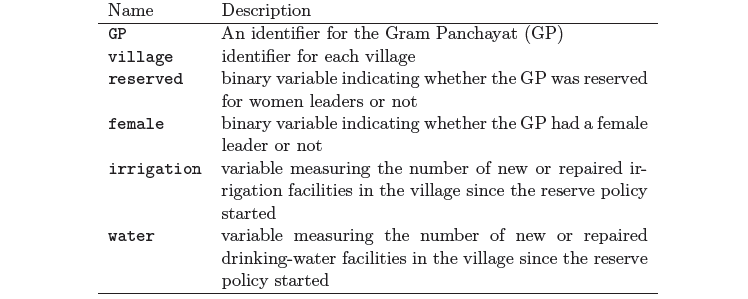
\includegraphics[width=1.1\textwidth]{women_desc.png}
\end{figure}		

\newpage
\begin{enumerate}
	\item [(a)] State a null and alternative (two-tailed) hypothesis. 
	
	\textbf{Null hypothesis:} The reservation policy does not affect the number of new or 
	repaired drinking water facilities in the villages. 
	
	\textbf{Alternative hypothesis:} The reservation policy affects the number of new or
	repaired drinking water facilities in the villages.
	
	\item [(b)] Run a bivariate regression to test this hypothesis in \texttt{R} (include your code!).
		
	First, I subset the variables "reserved" and "water" from the data set.			
		\lstinputlisting[language=R, firstline=129, lastline=129]{PS02_VD_17341481.R}  	
		
	Then, I calculated the slope ($\beta$) and the intercept ($\alpha$) by hand.
	
		\lstinputlisting[language=R, firstline=133, lastline=138]{PS02_VD_17341481.R}  	
		
	This returned the values $\beta = 9.25$ and $\alpha = 14.74$
	
	I checked my results: 
	
		\lstinputlisting[language=R, firstline=141, lastline=141]{PS02_VD_17341481.R}  	
		
	They seemed to be correct.
	
	Calculating the standard deviation: 
	
		\lstinputlisting[language=R, firstline=146, lastline=151]{PS02_VD_17341481.R}  	
	This gave me the value 33.45.
		
	The standard errors for $\beta$ and $\alpha$
	
		\lstinputlisting[language=R, firstline=155, lastline=155]{PS02_VD_17341481.R}  	
		\lstinputlisting[language=R, firstline=159, lastline=160]{PS02_VD_17341481.R}  	
	
	The standard error was 3.95 for $\beta$ and 2.29 for $\alpha$
	
	\newpage
	
	Calculating the Test statistic and P-value:
	
		\lstinputlisting[language=R, firstline=164, lastline=165]{PS02_VD_17341481.R}  	
	
	\begin{verbatim}
		[1] 0.01970398
		[1] 4.216474e-10
	\end{verbatim}
	
	I checked my results:
		\lstinputlisting[language=R, firstline=168, lastline=168]{PS02_VD_17341481.R}  	
	And they appear to match.
	
	\begin{verbatim}
		Call:
		lm(formula = EconRW$water ~ EconRW$reserved, data = EconRW)
		
		Residuals:
		Min      1Q  Median      3Q     Max 
		-23.991 -14.738  -7.865   2.262 316.009 
		
		Coefficients:
		             	  Estimate  Std. Error 	t value		Pr(>|t|)    
		(Intercept)       14.738      2.286   6.446 4.22e-10 ***
		EconRW$reserved    9.252      3.948   2.344   0.0197 *  
		---
		Signif. codes:  0 ‘***’ 0.001 ‘**’ 0.01 ‘*’ 0.05 ‘.’ 0.1 ‘ ’ 1
		
		Residual standard error: 33.45 on 320 degrees of freedom
		Multiple R-squared:  0.01688,	Adjusted R-squared:  0.0138 
		F-statistic: 5.493 on 1 and 320 DF,  p-value: 0.0197
	\end{verbatim}


	\item [(c)] Interpret the coefficient estimate for reservation policy. 
	
	The bivariate regression test showed statistically significant results with a p-value of 0.019. This is lower than the typical threshold of 0.05. The slope of the regression line was 9.252, showing a positive correlation. This suggests that having a reserved position for a female politician is associated with an average increase of 9.252 in new or repaired water facilities. 
	
\end{enumerate}

\end{document}
